\documentclass[conference]{IEEEtran}
\IEEEoverridecommandlockouts

\usepackage{cite}
\usepackage{amsmath,amssymb,amsfonts}
\usepackage{algorithmic}
\usepackage{graphicx}
\usepackage{textcomp}
\usepackage{xcolor}
\usepackage[hyphens]{url}
\usepackage{tikz}
\usepackage{dblfloatfix}
\usepackage{array}
\usetikzlibrary{shapes,arrows,positioning,fit,backgrounds}

\def\BibTeX{{\rm B\kern-.05em{\sc i\kern-.025em b}\kern-.08em
		T\kern-.1667em\lower.7ex\hbox{E}\kern-.125emX}}

\begin{document}
	
	\title{Raspberry Pi Robotics Extension Board}
	
	\author{
		\begin{tabular}{ccc}
			\begin{tabular}[t]{c}
				\textsuperscript{1\text{st}} Christian Kargl \\
				\textit{HTL St.P\"olten} \\
				St. P\"olten, Austria \\
				christian.kargl21@gmail.com
			\end{tabular}
			&
			\begin{tabular}[t]{c}
				\textsuperscript{2\text{nd}} Peter Strommer \\
				\textit{HTL St.P\"olten} \\
				St. P\"olten, Austria \\
				p.strommer@outlook.at
			\end{tabular}
			&
			\begin{tabular}[t]{c}
				\textsuperscript{3\text{rd}} Christoph Hackl \\
				\textit{HTL St.P\"olten} \\
				St. P\"olten, Austria \\
				christoph.hackl@htlstp.at
			\end{tabular}
		\end{tabular}
		\\[1em]
		\begin{tabular}{cc}
			\begin{tabular}[t]{c}
				\textsuperscript{4\text{th}} Moritz Klein \\
				\textit{HTL St.P\"olten} \\
				St. P\"olten, Austria \\
				moritzklein0810@gmail.com
			\end{tabular}
			&
			\begin{tabular}[t]{c}
				\textsuperscript{5\text{th}} Manuel Bichl \\
				\textit{HTL St.P\"olten} \\
				St. P\"olten, Austria \\
				manuel.bichl@htlstp.at
			\end{tabular}
		\end{tabular}
	}
	
	\maketitle
	
	\begin{abstract}
		This paper presents the development of a custom Raspberry Pi extension board for use in the European Conference on Educational Robotics (ECER). Instead of relying on separate add-on modules, the design combines motor control, servo control, and sensor interfacing on a single printed circuit board (PCB). The resulting hardware increases the number of available motor and servo outputs while reducing integration effort. Flexibility and expandability were key requirements throughout the design process, ensuring that the platform remains useful beyond the competition and can serve as a basis for future robotics projects.
	\end{abstract}
	
	\begin{IEEEkeywords}
		Robotics Controller, Raspberry Pi, Motor Driver, Servo Control, Educational Robotics
	\end{IEEEkeywords}
	
	\section{Introduction}
	
	Robotics competitions such as ECER demand hardware that is both reliable and adaptable under uncertain conditions. Single-board computers like the Raspberry Pi are attractive for such systems because they combine processing power, community support, and software flexibility \cite{b1}. However, competition robots also require actuator control, analog sensing, and robust power distribution, which are not provided directly by the Raspberry Pi itself.
	
	This paper presents a custom Raspberry Pi extension board developed for these requirements. The design integrates motor interfaces, servo control, sensor connectivity, inertial sensing, and power distribution into a single PCB, with the goal of reducing wiring complexity and improving integration compared with a modular controller setup.
	
	The hardware platform has also been upgraded significantly. Where the previous system was based on a Raspberry Pi~3, the new design uses a Raspberry Pi~5 with 16\,GB of RAM. An AI accelerator \cite{b3} capable of up to 26 tera operations per second (TOPS) complements the platform, enabling more neural-network-based approaches.
	
	\section{Related Work}
	
	\subsection{Overview of Existing Controller Approaches}
	
	In previous years, the Wombat controller was used as the central robotics platform in the ECER competition. The Wombat is an established educational robot controller with its own software environment and hardware ecosystem \cite{b7}. For the requirements of our previous competition setup, however, its built-in interfaces were no longer sufficient on their own.
	
	To overcome these limitations, supplementary boards were added to the Wombat in the previous project, including a servo shield and a GPIO expander \cite{b2}. This approach was functional, but it also increased wiring complexity, reduced mechanical robustness, and distributed related subsystems across several modules.
	
	The present work follows a different approach by integrating the required robotics interfaces directly onto a dedicated Raspberry Pi extension board. Instead of extending the existing controller step by step, the new design consolidates everything on one hardware platform.
	
	\section{Concept}
	
	\subsection{Design Goals}
	
	Because the exact competition tasks are not disclosed in advance, the design was intended to support a wide range of robot configurations. The main goals were to reduce wiring complexity, integrate the most important robotics interfaces on a single board, and separate high-level software execution from time-critical control tasks.
	
	More specifically, the platform was intended to provide the following capabilities:
	
	\begin{itemize}
		\item up to six motor outputs for robot locomotion
		\item eight servo outputs controlled through a dedicated Inter-Integrated Circuit (I\textsuperscript{2}C) servo controller \cite{b9}
		\item five digital sensor interfaces and analog acquisition through three single-ended and two differential analog channels
		\item onboard inertial measurement units
		\item separate power paths for logic electronics and high-current actuators
	\end{itemize}
	
	\subsection{Embedded Robotics Constraints}
	
	While the Raspberry Pi provides a flexible software platform, it does not provide native analog inputs, cannot drive motors directly, and is not intended for deterministic real-time actuator control. These limitations motivate the use of a dedicated extension board and an additional microcontroller for time-critical tasks.
	
	\begin{figure*}[!t]
		\centering
		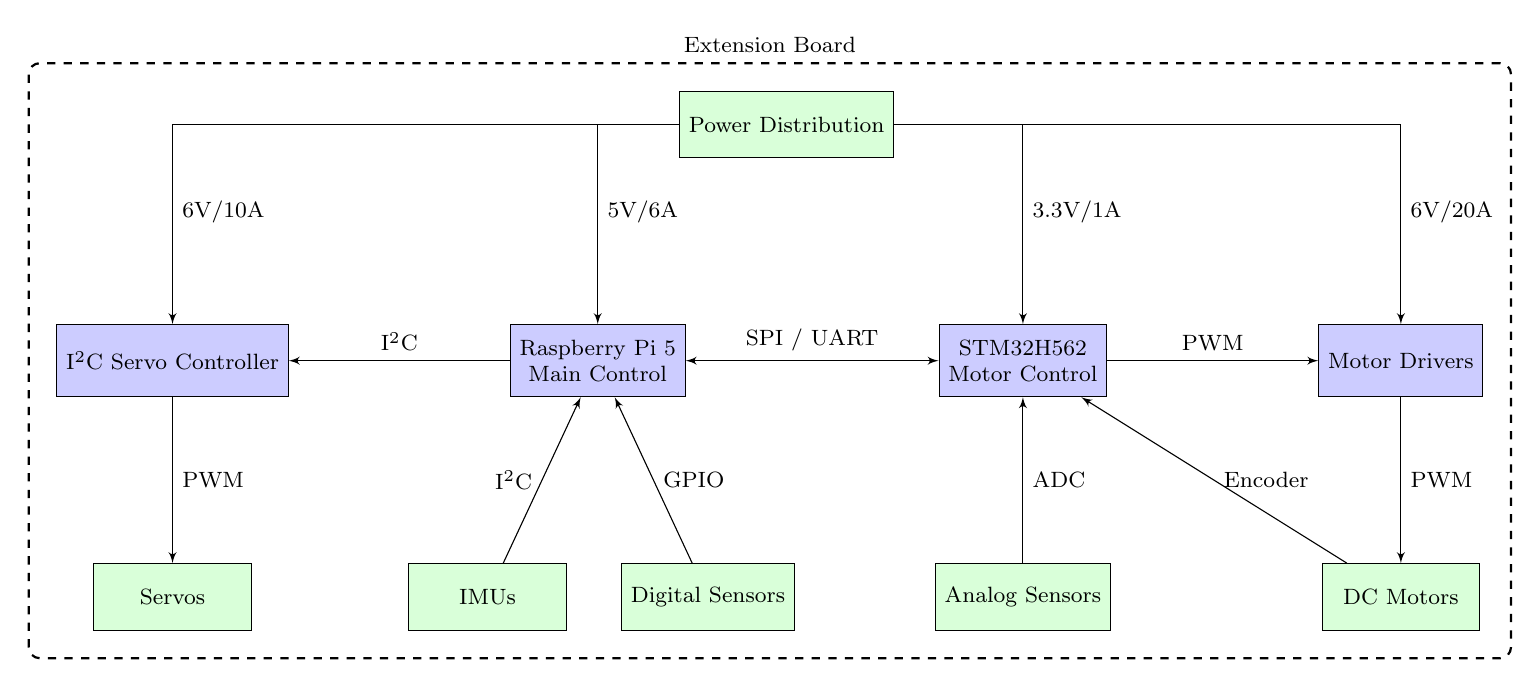
\begin{tikzpicture}[auto, font=\footnotesize]
			\tikzstyle{block} = [draw, fill=blue!20, rectangle,
			minimum height=2.6em, minimum width=2cm, align=center]
			\tikzstyle{io} = [draw, fill=green!15, rectangle,
			minimum height=2.4em, minimum width=2cm, align=center]
			\tikzstyle{line} = [draw, -latex']
			\tikzstyle{boardbox} = [draw, rounded corners, thick, dashed, inner sep=0.35cm]
			\node [io] (power) at (7.8,3.0) {Power Distribution};
			\node [io] (imu) at (4,-3.0) {IMUs};
			\node [block] (rpi) at (5.4,0) {Raspberry Pi 5\\Main Control};
			\node [block] (stm) at (10.8,0) {STM32H562\\Motor Control};
			\node [block] (motor) at (15.6,0) {Motor Drivers};
			\node [io] (motors) at (15.6,-3.0) {DC Motors};
			\node [block] (servoctl) at (0,0) {I\textsuperscript{2}C Servo Controller};
			\node [io] (digital) at (6.8,-3.0) {Digital Sensors};
			\node [io] (analog) at (10.8,-3.0) {Analog Sensors};
			\node [io] (servos) at (0,-3.0) {Servos};
			
			\draw [line] (power) -| node[pos=0.72, right] {5V/6A} (rpi);
			\draw [line] (power) -| node[pos=0.72, right] {3.3V/1A} (stm);
			\draw [line] (power) -| node[pos=0.72, right] {6V/20A} (motor);
			\draw [line] (power) -| node[pos=0.72, right] {6V/10A} (servoctl);
			\draw [line] (imu) -- node[left] {I\textsuperscript{2}C} (rpi);
			\draw [<->, >=latex'] (rpi) -- node[above] {SPI / UART} (stm);
			\draw [line] (stm) -- node[above] {PWM} (motor);
			\draw [line] (motor) -- node[right] {PWM}(motors);
			\draw [line] (motors) -- node[right] {Encoder} (stm);
			\draw [line] (servoctl) -- node[right] {PWM} (servos);
			\draw [line] (rpi) -- node[above] {I\textsuperscript{2}C} (servoctl);
			\draw [line] (digital) -- node[right] {GPIO} (rpi);
			\draw [line] (analog) -- node[right] {ADC} (stm);
			\begin{scope}[on background layer]
				\node [boardbox, fit=(power) (imu) (rpi) (stm) (motor) (servoctl),
				label={[align=center]above:Extension Board}] {};
			\end{scope}
		\end{tikzpicture}
		\caption{Functional block diagram of the Raspberry Pi robotics extension board system.}
		\label{fig:block-diagram}
	\end{figure*}
	\newpage
	
	

	\section{Implementation}
	
	The Raspberry Pi remains the central processing unit of the robot, executing the main control software and handling high-level decision making. The extension board bridges this controller to the physical actuators and sensors.
	
	Figure~\ref{fig:block-diagram} illustrates the functional structure of the system. The Raspberry Pi acts as the central controller and communicates directly with the digital sensors, the inertial measurement units (IMUs), and the servo controller via I\textsuperscript{2}C. A dedicated microcontroller from STMicroelectronics (STM) is used only for time-critical motor control and analog sensor acquisition.

	
	\subsection{Motor Driver Interfaces}
	One of the primary functions of the board is the control of DC motors used for robot locomotion. Since direct motor actuation requires dedicated driver circuitry, motor driver stages are implemented on the extension board. In the current design, the motor stage is based on three DRV8411 motor drivers \cite{b10} and is designed for up to six motor outputs.
	
	These drivers provide the required actuation for the motors, while their control signals are generated by the STM microcontroller. Encoder feedback is available for all driven motors, enabling closed-loop motor control through the same microcontroller.
	
	\subsection{Servo Interfaces}
	
	Servos are one of the most important components in robotics.	
	The extension board therefore includes dedicated servo connectors that allow several servo motors to be connected directly to the board. Servo control is implemented through an I\textsuperscript{2}C-based servo controller addressed by the Raspberry Pi. In the current design, this function is realized using the PCA9685 PWM controller \cite{b9}, of which eight channels are currently assigned to servo outputs.
	
	\subsection{Sensor Interfaces}
	
	Robotic systems require sensors to detect environmental conditions. The extension board supports five digital sensor interfaces through GPIO connections as well as analog acquisition through three single-ended and two differential analog channels. The digital sensors are connected directly to the Raspberry Pi, while the analog sensors are connected via the STM microcontroller. The single-ended and differential analog channels are implemented as separate acquisition paths.
	
	\subsection{Inertial Measurement Units}
	
	In addition to the external sensor interfaces, the board also integrates onboard inertial measurement units. These IMUs provide motion and orientation data directly on the controller board and are connected to the Raspberry Pi via an I\textsuperscript{2}C interface for tasks such as stabilization and motion tracking.
	
	The current design includes a CEVA BNO085 \cite{b4} and an ST LSM6DSO \cite{b5}. Both devices are planned to operate via I\textsuperscript{2}C. By integrating these components directly on the PCB, the system gains immediate access to acceleration, angular rate, and orientation-related data without requiring additional external modules. Two different IMUs are used for redundancy.
	
	\subsection{Power Distribution}
	
	Motors and servos place significantly higher power demands on the system than the logic electronics. For this reason, the design includes a generously dimensioned power distribution stage for both logic electronics and high-power actuators.
	
	The board is supplied from a 12\,V input, corresponding to a 3S1P battery configuration. From this input, four buck converters generate the required lower supply voltages for the different subsystems.
	
	Three of these converters provide 6\,V at up to 10\,A. One 6\,V rail is used for the DC motors, while two separate 6\,V rails are dedicated to the servos. The servo power stages were intentionally dimensioned with a high current reserve in order to handle the high holding currents that can occur during operation.
	
	Another buck converter provides 5\,V at up to 6\,A for the Raspberry Pi. From this 5\,V rail, an additional conversion stage generates 3.3\,V for peripheral electronics such as the STM microcontroller, the IMUs, and other low-voltage components.
	
	Separate power paths are used for logic electronics and high-power actuators in order to reduce electrical disturbances and improve overall system stability.
	
	\section{Planned Motor Control Microcontroller}
	
	To handle time-critical tasks, the controller board includes an additional microcontroller, the STM32H562RIT6 \cite{b6}. This microcontroller is intended to handle all real-time motor control operations once firmware integration is completed.
	
	Motor control in robotics often requires deterministic timing and fast feedback processing. Because the Raspberry Pi runs a full operating system, it is not ideal for precise real-time control. The STM microcontroller is therefore intended to execute the complete motor control logic.
	
	The planned firmware for the microcontroller includes Proportional-Integral-Derivative (PID) control algorithms to regulate the motor speed and movement of the robot. In the intended architecture, the controller continuously reads feedback signals from the motor encoders and calculates the control output required to achieve the desired motor speed.
	
	Another important planned function of the microcontroller is handling analog sensors. Since the Raspberry Pi does not provide native analog inputs, analog sensor signals are connected directly to the microcontroller's Analog-to-Digital Converter (ADC) inputs. Some of these channels can also be used for differential measurements. In the intended system architecture, the measured values are then transferred to the Raspberry Pi.
	
	Communication between the Raspberry Pi and the STM microcontroller is planned to use a Serial Peripheral Interface (SPI). Through this interface the Raspberry Pi is intended to send commands such as motor speed targets and receive sensor data from the microcontroller.
	
	For development and debugging purposes, the microcontroller firmware was initially intended to be uploaded directly from the Raspberry Pi using a Universal Asynchronous Receiver-Transmitter (UART) connection. The available bootloader interfaces and their activation conditions are device-dependent and documented by STMicroelectronics in application note AN2606 \cite{b8}, while the USART bootloader protocol itself is described in AN3155 \cite{b11}. In the current prototype, difficulties with this flashing path led to a transition towards Serial Wire Debug (SWD) programming for more reliable firmware upload and debugging.
	
	\section{Results}
		
	At the current stage of the project, the controller board hardware has already been designed and assembled. The main components, including the Raspberry Pi interface, motor drivers, microcontroller, and sensor interfaces, are implemented on the board.
		
	Figure~\ref{fig:board-overview} shows the current PCB layout of the prototype board in its present development stage.
		
	Initial bring-up confirms correct power-up, the presence of the required 5\,V, 6\,V, and 3.3\,V supply rails, and successful Raspberry Pi operation. These results already validate the basic electrical design and the general power-distribution concept.
	
	On the Raspberry Pi side, several subsystems are already functional. The I\textsuperscript{2}C-based servo controller for all eight assigned servo channels operates as intended, all five digital sensor interfaces have been tested successfully, and one of the two integrated IMUs, the LSM6DSO, can already be detected and read out. This shows that the chosen architecture is viable in practice.
	
	The following table summarizes the current validation status of the most important subsystems.
	
	
	\begin{center}
		\textbf{Table I}\\
		Current subsystem status of the prototype board.
		
		\centering
		\begin{tabular}{|>{\raggedright\arraybackslash}p{2.4cm}|>{\raggedright\arraybackslash}p{1.8cm}|>{\raggedright\arraybackslash}p{2.4cm}|}
			\hline
			Subsystem & Status & Observation \\ \hline
			Power rails & Verified & 5\,V, 6\,V, and 3.3\,V rails present \\ \hline
			Raspberry Pi & Verified & System boots successfully on the board \\ \hline
			Servo control & Verified & All 8 PCA9685-based servo channels tested \\ \hline
			Digital sensors & Verified & All 5 GPIO-based sensor interfaces tested \\ \hline
			LSM6DSO & Verified & Device detected and sensor values read \\ \hline
			BNO085 & Open & Device not yet detected via I\textsuperscript{2}C \\ \hline
			STM flashing & Open & UART flashing not yet reliable \\ \hline
			Motor control & Open & Depends on STM32 programming and communication \\ \hline
		\end{tabular}
	\end{center}
		
	The main limitation of the current prototype is the incomplete STM integration. At the moment, the STM microcontroller cannot yet be programmed reliably through the intended UART flashing path, which also prevents validation of the SPI communication between the Raspberry Pi and the microcontroller. As a consequence, the three single-ended analog channels, the two differential analog channels, PWM-based motor control, and encoder processing for all motor channels could not yet be evaluated on the assembled board. Since the STM32 bootloader behavior and supported interfaces are device-specific \cite{b8}, the debugging workflow is currently being migrated to SWD programming.
	
	Further open issues include the missing detection of the BNO085 IMU and the absence of load tests for the power stage and actuator interfaces. These aspects currently limit the evaluation to basic bring-up and subsystem checks, but they also define the next validation steps.
	
	\section{Limitations and Future Work}
	
	The current paper focuses on the system architecture and hardware implementation of the first prototype, but it does not yet provide a full experimental evaluation. Future work will therefore include systematic validation of the motor control performance, communication reliability, IMU integration, and power stability under realistic operating conditions.
	
	In addition, the firmware and software stack will be extended to make better use of the integrated interfaces during real competition tasks. Once STM programming and communication are stable, quantitative measurements will be added to compare the new controller against the previously used modular Wombat-based setup.
	
	\begin{figure*}[!t]
		\centering
		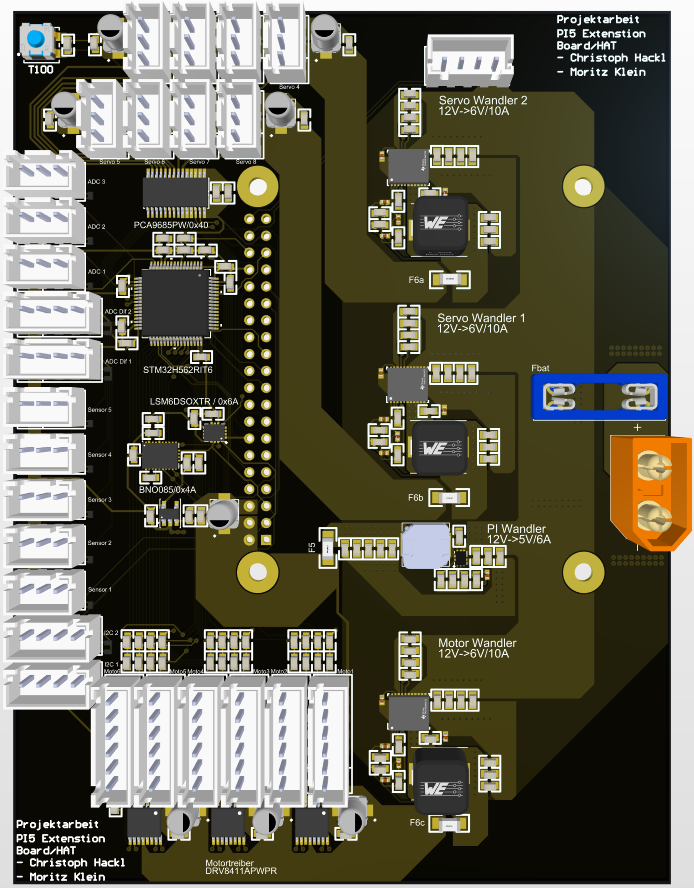
\includegraphics[width=0.97\textwidth]{Board.png}
		\caption{Current PCB layout of the Raspberry Pi robotics extension board prototype.}
		\label{fig:board-overview}
	\end{figure*}
	
	\section{Conclusion}
	
	This paper presented the development of a Raspberry Pi extension board for robotics applications in the ECER competition. The proposed design integrates motor drivers, servo interfaces, sensor connections, inertial sensing, and power distribution into a single hardware platform.
	
	Compared with the previously used modular Wombat-based setup, the new design reduces wiring complexity and provides a clearer separation between high-level processing on the Raspberry Pi and time-critical tasks on the STM microcontroller. Initial bring-up results already confirm the validity of the electrical design and several Raspberry Pi-side subsystems.
	
	Although the controller is still under development, the current prototype provides a solid basis for further validation, firmware integration, and future robotics projects.
	\newpage
	
	\begin{thebibliography}{00}
		
		\bibitem{b1}
		Raspberry Pi Ltd., 
		``Raspberry Pi 5 Product Brief,'' 
		2023. [Online]. Available: \url{https://pip-assets.raspberrypi.com/categories/892-raspberry-pi-5/documents/RP-008348-DS-6-raspberry-pi-5-product-brief.pdf}
		
		\bibitem{b2}
		C. Kargl, M. Bichl, P. Strommer, and C. Hackl, 
		``Extension Boards for the Wombat,'' 
		HTL St.~P\"olten Robotics Project Report, 2025.
		
		\bibitem{b3}
		Raspberry Pi Ltd.,
		``Raspberry Pi AI HAT Product Brief,''
		2024. [Online]. Available: \url{https://pip-assets.raspberrypi.com/categories/1081-raspberry-pi-ai-hat/documents/RP-008133-DS-1-raspberry-pi-ai-hat-plus-product-brief.pdf}
		
		\bibitem{b4}
		CEVA, 
		``BNO085 Smart Sensor Hub Datasheet,'' 
		2023. [Online]. Available: \url{https://www.ceva-ip.com/wp-content/uploads/BNO080_085-Datasheet.pdf}
		
		\bibitem{b5}
		STMicroelectronics, 
		``LSM6DSO IMU Datasheet,'' 
		2023. [Online]. Available: \url{https://www.st.com/resource/en/datasheet/lsm6dso.pdf}
		
		\bibitem{b6}
		STMicroelectronics, 
		``STM32H562xx Datasheet,'' 
		2024. [Online]. Available: \url{https://www.st.com/resource/en/datasheet/stm32h562ri.pdf}
		
		\bibitem{b7}
		KIPR,
		``KIPR Hardware/Software: KIPR Wombat,''
		[Online]. Available: \url{https://www.kipr.org/kipr/hardware-software}
		
		\bibitem{b8}
		STMicroelectronics,
		``AN2606: STM32 Microcontroller System Memory Boot Mode,''
		[Online]. Available: \url{https://www.st.com/resource/en/application_note/an2606-stm32-microcontroller-system-memory-boot-mode-stmicroelectronics.pdf}
		
		\bibitem{b9}
		NXP Semiconductors,
		``PCA9685: 16-Channel, 12-Bit PWM Fm+ I\textsuperscript{2}C-Bus LED Controller,''
		[Online]. Available: \url{https://www.nxp.com/docs/en/data-sheet/PCA9685.pdf}
		
		\bibitem{b10}
		Texas Instruments,
		``DRV8411 11-V to 50-V, 7-A Peak H-Bridge Motor Driver,''
		[Online]. Available: \url{https://www.ti.com/lit/ds/symlink/drv8411.pdf?ts=1775644197177}
		
		\bibitem{b11}
		STMicroelectronics,
		``AN3155: USART Protocol Used in the STM32 Bootloader,''
		[Online]. Available: \url{https://www.st.com/resource/en/application_note/an3155-usart-protocol-used-in-the-stm32-bootloader-stmicroelectronics.pdf}
		
		
	\end{thebibliography}
	
	
\end{document}
